% Deterministic pruning example. The solid teal K_4 survives; dashed edges
% touch vertices deleted in the first two simultaneous pruning rounds.
% This source is a single-column graphic; its caption belongs in the section.
\begingroup
\definecolor{coreteal}{RGB}{33,112,117}
\definecolor{prunegray}{RGB}{150,156,160}
\definecolor{pruneorange}{RGB}{182,112,49}
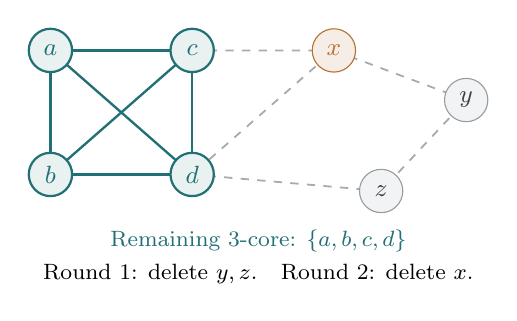
\begin{tikzpicture}[
  x=1.2cm, y=1.05cm,
  vertex/.style={circle, minimum size=5.5mm, inner sep=0pt, font=\small},
  retained/.style={vertex, draw=coreteal, fill=coreteal!10, text=coreteal,
    line width=0.8pt},
  first/.style={vertex, draw=prunegray, fill=prunegray!12, text=black!75},
  second/.style={vertex, draw=pruneorange, fill=pruneorange!12,
    text=pruneorange},
  core edge/.style={draw=coreteal, line width=0.85pt},
  deleted edge/.style={draw=prunegray!85, dashed, line width=0.65pt}
]
  % Six edges on a,b,c,d form K_4, so every retained vertex has degree three.
  \coordinate (a) at (0,1);
  \coordinate (b) at (0,-0.5);
  \coordinate (c) at (1.5,1);
  \coordinate (d) at (1.5,-0.5);
  \coordinate (x) at (3,1);
  \coordinate (y) at (4.4,0.4);
  \coordinate (z) at (3.5,-0.7);
  \draw[core edge] (a)--(b)--(d)--(c)--(a);
  \draw[core edge] (a)--(d) (b)--(c);
  % Initially y,z have degree two, whereas x has degree three. Removing
  % y,z leaves x with only c,d, so x is removed in the next round.
  \draw[deleted edge] (c)--(x)--(d) (x)--(y)--(z)--(d);
  \foreach \v in {a,b,c,d} \node[retained] at (\v) {$\v$};
  \node[second] at (x) {$x$};
  \foreach \v in {y,z} \node[first] at (\v) {$\v$};
  \node[font=\footnotesize, text=coreteal] at (2.2,-1.3)
    {Remaining 3-core: $\{a,b,c,d\}$};
  \node[font=\footnotesize] at (2.2,-1.7)
    {Round 1: delete $y,z$.\quad Round 2: delete $x$.};
\end{tikzpicture}
\endgroup
